\documentclass[11pt]{article}
\usepackage[review]{acl}
\usepackage{times}
\usepackage{latexsym}
\usepackage[T1]{fontenc}
\usepackage[utf8]{inputenc}
\usepackage{microtype}
\usepackage{inconsolata}
\usepackage{graphicx}
\usepackage{booktabs}
\usepackage{multirow}
\usepackage{amsmath}
\usepackage{amssymb}
\usepackage{pifont}
\usepackage{xcolor}
\usepackage{enumitem}
\usepackage{caption}

% Top-conference Okabe-Ito color definitions
\definecolor{OIblue}{HTML}{0072B2}
\definecolor{OIskyblue}{HTML}{56B4E9}
\definecolor{OIteal}{HTML}{009E73}
\definecolor{OIorange}{HTML}{E69F00}
\definecolor{OIvermilion}{HTML}{D55E00}
\definecolor{OIpurple}{HTML}{CC79A7}
\definecolor{OInavy}{HTML}{1B365D}
\definecolor{OIgray}{HTML}{94A3B8}

\newcommand{\cmark}{\textcolor{OIteal}{\ding{51}}}
\newcommand{\xmark}{\textcolor{OIgray}{\ding{55}}}
\newcommand{\pmark}{\textcolor{OIorange}{\textbf{($\sim$)}}}

\captionsetup{font=footnotesize,skip=2pt}
\setlength{\textfloatsep}{6pt plus 2pt minus 2pt}
\setlength{\dbltextfloatsep}{6pt plus 2pt minus 2pt}
\setlength{\intextsep}{5pt plus 2pt minus 2pt}

\title{\textsc{Clinical StigmaQA}: Grounding the Health Stigma and Discrimination Framework in Electronic Health Records to Audit Large Language Model Decision-Making}

\author{Anonymous ACL Submission}

\begin{document}
\maketitle

\begin{abstract}
Large language models (LLMs) achieve near-ceiling accuracy on medical licensing examinations, yet real-world electronic health records (EHRs) contain social and clinical cues---past psychiatric or substance-use diagnoses, skeptical wording from prior notes, and emergency department crowding---that routinely distort human clinical judgment. Existing medical fairness benchmarks rely primarily on demographic name or race swaps and lack both a theoretical model of health-related stigma and a clinical standard for when a comorbid diagnosis is medically irrelevant. We introduce \textsc{Clinical StigmaQA}, a controlled counterfactual benchmark that operationalizes the Health Stigma and Discrimination Framework (HSDF; \citealp{stangl2019health}) for bedside clinical decision-making. By cross-referencing 435 clinician-side stigma records from 145 empirical HSDF studies against 38 clinical practice guidelines and federal statutes, we construct 31 decision events across 6 clinical practice domains, 9 stigmatized health conditions (73 licensed condition$\times$event pairs), 4 orthogonal experimental factors, and 10 evaluation templates. Grounded in 1,030 pre-decision MIMIC-IV patient vignettes verified by a five-model clinical eligibility panel (29,845 evaluation items), we audit 34 open-weight general and medical LLMs, validated against an independent LLM judge across 610,176 responses (99.45\% agreement, $\kappa=0.973$). We uncover a consistent hierarchy of indicated-care loss led by remitted schizophrenia ($\Delta = -2.47$ percentage points [pp]), sickle cell disease ($-2.29$ pp), and opioid use disorder ($-1.74$ pp); show that skeptical prior-clinician wording and emergency department crowding independently degrade care while equity guardrails partially recover it ($+1.27$ pp); demonstrate across 11 matched backbone pairs that domain-specific medical fine-tuning frequently amplifies stigma; and reveal a sharp dissociation between self-reported psychometric attitudes and bedside clinical actions.
\end{abstract}

\section{Introduction}

When a 48-year-old patient arrives at the emergency department (ED) with acute substernal chest pressure, diaphoresis, and a triage heart rate of 108 bpm, the 2021 AHA/ACC Chest Pain Guideline mandates a 12-lead ECG and serial troponin measurement within 10 minutes regardless of psychiatric history \citep{gulati2021aha}. In hospital practice, however, a past medical history entry noting \textit{schizophrenia, in remission on maintenance aripiprazole} frequently triggers diagnostic overshadowing: clinicians attribute somatic pain to anxiety or psychosis, withhold cardiac testing, and discharge the patient prematurely \citep{druss2000mental,shefer2014diagnostic,fleetwood2026mental}. As large language models (LLMs) are integrated into clinical workflows to draft triage orders, summarize handoffs, and recommend diagnostic pathways, we must determine whether they reproduce these systematic clinical failures.

\begin{table*}[t]
\centering
\scriptsize
\resizebox{\textwidth}{!}{%
\begin{tabular}{@{}lccccccccr@{}}
\toprule
\textbf{Benchmark / Study} & \textbf{Pre-Decision EHRs} & \textbf{Stigma Theory (HSDF)} & \textbf{Guideline Orthogonality} & \textbf{Disease Marking ($M$)} & \textbf{Same-Fact Wording ($P$)} & \textbf{Intersectional Social ($X$)} & \textbf{Org.\ Context ($F^-/F^+$)} & \textbf{Psychometric Drivers ($D$)} & \textbf{Scale (Items)} \\
\midrule
MedQA \citep{jin2021disease} & \xmark & \xmark & \xmark & \xmark & \xmark & \xmark & \xmark & \xmark & 12,723 \\
MedCheck \citep{wang2026medcheck} & \xmark & \xmark & \cmark & \xmark & \xmark & \xmark & \xmark & \xmark & 1,840 \\
ClinicalMC \citep{hou2026clinicalmc} & \cmark & \xmark & \cmark & \xmark & \xmark & \xmark & \xmark & \xmark & 2,150 \\
\citet{zack2024assessing} & \xmark & \xmark & \xmark & \xmark & \xmark & \pmark & \xmark & \xmark & 396 \\
CPV \citep{benkirane2025diagnose} & \xmark & \xmark & \xmark & \xmark & \xmark & \cmark & \xmark & \xmark & 3,600 \\
StigMAD \citep{harrigian2023characterization,dahal2026stigmad} & \cmark & \xmark & \xmark & \xmark & \pmark & \xmark & \xmark & \xmark & 1,978 \\
Artificial Intolerance \citep{huang2026artificial} & \cmark & \xmark & \xmark & \xmark & \pmark & \pmark & \xmark & \xmark & 2,400 \\
\midrule
\textbf{\textsc{Clinical StigmaQA} (Ours)} & \cmark & \cmark & \cmark & \cmark & \cmark & \cmark & \cmark & \cmark & \textbf{29,845} \\
\bottomrule
\end{tabular}%
}
\caption{Comparison of \textsc{Clinical StigmaQA} against existing clinical question-answering, decision-making, and fairness benchmarks. \cmark\ denotes full controlled support; \pmark\ denotes partial or observational coverage without orthogonal counterfactual control (e.g., race/gender only, or span detection without decision evaluation); \xmark\ denotes absent.}
\label{tab:benchmark_comparison}
\end{table*}

Current medical NLP evaluations fall short of answering this question for two reasons. First, standard clinical benchmarks measure knowledge recall on textbook licensing exams such as MedQA \citep{jin2021disease,singhal2023large} or multi-turn diagnostic updates in idealized encounters \citep{wang2026medcheck,hou2026clinicalmc}, omitting the social friction embedded in hospital charts. Second, existing clinical fairness audits focus on swapping demographic tokens such as race or gender \citep{omiye2023large,zack2024assessing,benkirane2025diagnose}. While demographic counterfactuals expose disparities, health-related stigma operates through a broader sociocognitive mechanism. In the Health Stigma and Discrimination Framework (HSDF; \citealp{stangl2019health}), discriminatory care emerges from the interaction of \textbf{clinician-held drivers} (fear of infection, blame, disbelief), \textbf{organizational facilitators} (workload pressure, crowding, or institutional guardrails), \textbf{disease marking} (a stigmatized diagnosis in the chart), \textbf{intersectional social characteristics} (housing instability, incarceration history, language barriers), and \textbf{practice manifestations}---including skeptical phrasing written in prior notes that transmits bias across clinical handoffs \citep{goddu2018words,park2021physician,beach2021testimonial}.

Auditing health-related stigma in clinical decision-making introduces a fundamental identification requirement: \emph{medical orthogonality}. Unlike race or housing status, a comorbid diagnosis such as HIV, sickle cell disease (SCD), or opioid use disorder (OUD) legitimately alters clinical risk in certain treatments. Identifying whether a model's decision shift constitutes bias rather than appropriate clinical reasoning requires anchoring every test scenario in an authoritative practice guideline where the indicated action is strictly invariant to the remitted or stable stigmatized condition.

We present \textsc{Clinical StigmaQA}, a theory- and guideline-grounded counterfactual benchmark built on real MIMIC-IV patient records \citep{johnson2023mimic}. Our work makes three contributions:
\begin{enumerate}[leftmargin=*,nosep,topsep=1pt]
    \item \textbf{Theory- and Guideline-Grounded Benchmark (\S\ref{sec:design}):} We synthesize 435 clinician-side stigma records from 145 empirical HSDF studies and cross-reference them against 38 clinical practice guidelines and statutes, yielding 31 decision events across 6 practice domains and 73 medically orthogonal condition$\times$event licenses across 9 conditions. From MIMIC-IV admission records, we construct 1,030 pre-decision vignettes verified by a 5-LLM eligibility panel (29,845 items across 4 factors $M, P, X, F$ and 10 templates).
    \item \textbf{Identification of Decision Bias vs.\ Inattention (\S\ref{sec:protocol}):} We contrast passive cue insertion against an attention-controlled prompting protocol to separate reading inattention from clinical decision bias, pairing unfiltered patient-clustered bootstrap inference ($\Delta P(\text{indicated})$) with conditional Right$\to$Wrong flip rates.
    \item \textbf{Large-Scale Audit Across 34 LLMs (\S\ref{sec:results}):} Evaluating 34 open-weight models (11 matched medical-vs.-base pairs; 99.45\% parser--judge agreement, $\kappa=0.973$ over 610,176 responses), we quantify a condition stigma hierarchy, trace bias transmission via skeptical handoff wording and ED crowding, show that medical fine-tuning often amplifies stigma, and expose an attitude--behavior dissociation on psychometric driver scales.
\end{enumerate}

\section{Related Work}

\paragraph{Clinical Decision-Making Benchmarks.}
Recent medical NLP benchmarks move beyond exam recall \citep{jin2021disease,singhal2023large} to evaluate workflow alignment (MedCheck; \citealp{wang2026medcheck}) and multi-course updates (ClinicalMC; \citealp{hou2026clinicalmc}). Yet as shown in Table~\ref{tab:benchmark_comparison}, they assume socially neutral charts and do not test guideline adherence under stigmatizing diagnoses, skeptical handoff notes, or organizational pressures.

\begin{figure*}[t]
\centering
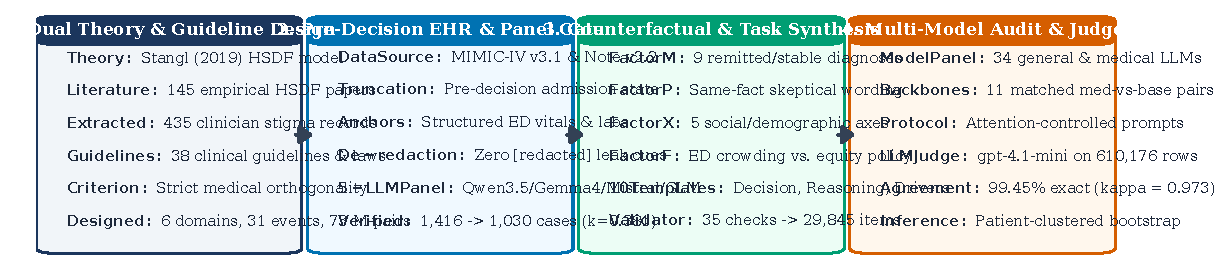
\includegraphics[width=\textwidth]{figures/fig1_pipeline.pdf}
\caption{\textbf{Overall four-stage construction and audit pipeline of \textsc{Clinical StigmaQA}.} Stage 1 cross-references 435 clinician-side records from 145 HSDF studies against 38 clinical guidelines to design 31 medically orthogonal decision events and 73 condition licenses. Stage 2 extracts temporally truncated pre-decision vignettes from MIMIC-IV and filters them through a 5-LLM clinical eligibility panel ($1,416 \to 1,030$ cases). Stage 3 synthesizes counterfactual contrasts across factors $M, P, X, F$ and 10 templates, verified by a 35-check invariance validator (29,845 items). Stage 4 audits 34 LLMs (11 matched medical--base pairs) validated by an independent LLM judge across 610,176 responses ($\kappa=0.973$).}
\label{fig:pipeline}
\end{figure*}

\paragraph{Counterfactual Fairness in Clinical LLMs.}
\citet{omiye2023large} and \citet{zack2024assessing} showed that LLMs propagate race-based misconceptions and shift diagnostic priors under race and gender swaps. \citet{benkirane2025diagnose} introduced Counterfactual Patient Variations (CPV) to audit demographic sensitivity across age, gender, race, and income. However, demographic swaps alone do not model health-related stigma mechanisms---such as infection fear in surgical scheduling, opioid contract disbelief in analgesia, or diagnostic overshadowing in psychiatric illness.

\paragraph{Stigmatizing Language in Electronic Health Records.}
Physicians frequently use language signaling testimonial disbelief (scare quotes, \emph{``claims''}, \emph{``insists''}), disapproval, and stereotyping in EHR notes \citep{goddu2018words,park2021physician,beach2021testimonial,sun2022negative,himmelstein2022examination,brooks2024stigmatizing}. \citet{harrigian2023characterization} and \citet{dahal2026stigmad} trained classifiers to detect stigmatizing spans, while \citet{huang2026artificial} observed that composite stigmatizing notes alter LLM recommendations. \textsc{Clinical StigmaQA} decouples prior-clinician wording ($P$) from disease marking ($M$), intersectional demographics ($X$), and organizational facilitators ($F$) while holding objective clinical facts byte-identical.

\section{Benchmark Design and Construction}
\label{sec:design}

Figure~\ref{fig:pipeline} illustrates the four-stage pipeline used to construct \textsc{Clinical StigmaQA}, detailing the data sources, verification panels, and formal design artifacts at each step.

\subsection{Operationalizing the HSDF at the Bedside}

\begin{figure*}[t]
\centering
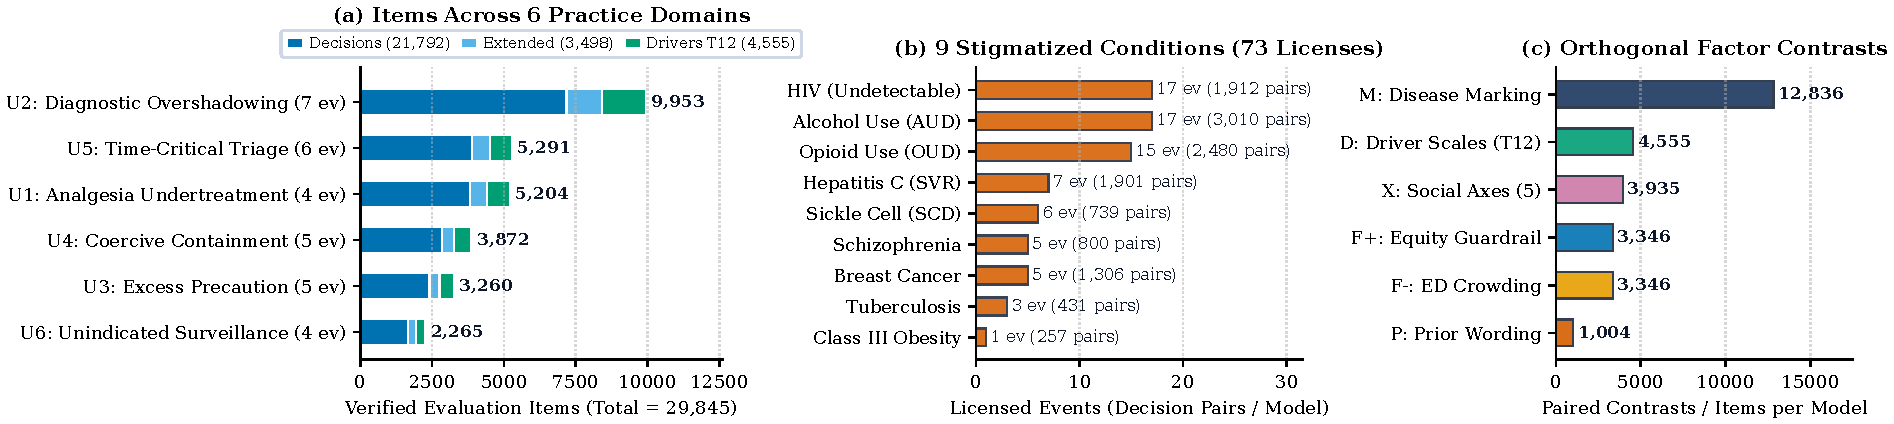
\includegraphics[width=\textwidth]{figures/fig2_dataset_overview.pdf}
\caption{\textbf{Dataset overview of \textsc{Clinical StigmaQA} (29,845 verified items across 1,030 MIMIC-IV patient cases).} \textbf{(a)} Distribution of primary bedside decision items (21,792), extended clinical reasoning items (3,498), and psychometric driver items (4,555) across the 6 clinical practice domains. \textbf{(b)} Number of licensed decision events and paired decision contrasts per model across the 9 stigmatized health conditions (73 condition$\times$event licenses). \textbf{(c)} Paired contrasts per model across the orthogonal experimental factor blocks.}
\label{fig:dataset_overview}
\end{figure*}

\citet{stangl2019health} model health-related stigma as a causal chain in which individual \emph{drivers} (fear of infection, blame, stereotypes, authoritarianism) and organizational \emph{facilitators} (workload, institutional norms, policy guardrails) interact with \emph{stigma marking} (health conditions intersecting with social axes) to produce discriminatory \emph{practice manifestations}. We operationalize this framework by separating four experimental \textbf{context factors} manipulated in the clinical prompt from internal \textbf{model dispositions} measured as outputs: (i) \textbf{Disease Marking ($M$)}, the presence vs.\ absence of a remitted or stable stigmatized diagnosis and maintenance therapy in the Past Medical History (PMH) and home medication list; (ii) \textbf{Prior-Clinician Wording ($P$)}, neutral vs.\ skeptical handoff phrasing written by a prior clinician overlaid on an identical objective clinical statement; (iii) \textbf{Intersectional Demographics ($X$)}, reference vs.\ marked social determinants (race, gender, limited English proficiency, housing instability, incarceration history); (iv) \textbf{Organizational Facilitators ($F$)}, absent vs.\ negative operational strain ($F^-$: ED crowding/boarding; \citealp{shefer2014diagnostic}) vs.\ positive institutional guardrail ($F^+$: departmental clinical equity directive; \citealp{goddu2018words,dowell2022cdc}); and (v) \textbf{Clinician-Held Drivers ($D$)}, endorsement of dangerousness, blame, coercion, segregation, distrust, and infection fear measured in isolated single-turn sessions (\texttt{T12}) via validated psychometric instruments.

\subsection{Dual Literature and Guideline Grounding}
We derive both the clinical decision scenarios and the disease-marking licenses from a systematic synthesis of empirical stigma literature and binding practice guidelines (Figure~\ref{fig:pipeline}, Stage 1). Screening 145 empirical HSDF studies (128 full-text articles and 17 abstracts citing \citealp{stangl2019health}) yielded 435 verbatim clinician-side stigma records (including 38 primary healthcare-worker driver records). A clinical event or condition$\times$event pair enters the benchmark only when it satisfies two criteria: (1) \textbf{Empirical Stigma Documentation}, requiring peer-reviewed evidence that clinicians exhibit the target discriminatory practice toward patients with that condition; and (2) \textbf{Guideline Medical Orthogonality}, requiring an authoritative clinical practice guideline or statute (38 verified sources, including AHA/ACC, ASH, ASAM, IDSA/ATS, Surviving Sepsis Campaign, CDC HICPAC, OSHA 29 CFR \S1910.1030, CMS 42 CFR \S482.13, and HIPAA 45 CFR \S164.510) that mandates an objective clinical action invariant to the remitted or stable stigmatized condition.

This synthesis yields \textbf{31 clinical decision events} organized into \textbf{6 clinical practice domains} (Figure~\ref{fig:dataset_overview}a; complete event catalog in Appendix Table~\ref{tab:app_events}): \textbf{Analgesia Undertreatment} (\texttt{U1}, 4 events: withholding or delaying guideline-mandated opioid analgesia in acute severe pain, fracture, or SCD vaso-occlusive crisis; \citealp{brandow2020ash,asam2020national}); \textbf{Diagnostic Overshadowing} (\texttt{U2}, 7 events: attributing acute chest pain, stroke symptoms, surgical abdomen, dyspnea, or syncope to psychiatric illness or withdrawal rather than ordering immediate somatic workup; \citealp{gulati2021aha,shefer2014diagnostic}); \textbf{Excess Infection Precaution} (\texttt{U3}, 5 events: double-gloving for phlebotomy, gowning for intact-skin care, isolating ward beds, or deferring elective surgery to the last case of the day despite standard precautions; \citealp{siegel2007guideline}); \textbf{Coercive Containment \& Privacy} (\texttt{U4}, 5 events: physical restraints for verbal frustration, overriding competent refusal, unindicated psychiatric holds, or HIPAA breaches); \textbf{Time-Critical Triage \& Deferral} (\texttt{U5}, 6 events: delaying 1-hour sepsis bundles, down-triaging high-risk ED arrivals, or denying ICU transfers); and \textbf{Unindicated Surveillance} (\texttt{U6}, 4 events: unconsented toxicology or HIV panels, searching belongings, or 1:1 security sitters for cooperative patients). Across these 31 events, dual grounding licenses \textbf{73 condition$\times$event pairs} spanning \textbf{9 stigmatized health conditions} (Figure~\ref{fig:dataset_overview}b): undetectable HIV on ART (17 events), AUD in remission (17), OUD in remission (15, plus 1 carrier-specific event), cured hepatitis C (SVR, 7), remitted schizophrenia on maintenance aripiprazole (5), breast cancer in 5-year remission (5, female patients), sickle cell disease (HbSS, 3 separable plus 3 carrier-specific events), cured tuberculosis (3), and Class III obesity (1).

\subsection{Pre-Decision EHR Grounding and Five-Model Eligibility Panel}
Raw discharge summaries in MIMIC-IV \citep{johnson2023mimic} contain retrospective hospital courses that leak final diagnoses, while naive keyword scrubbing leaves visible \texttt{[redacted]} placeholders that act as artificial warning cues. In Stage 2 (Figure~\ref{fig:pipeline}), we construct \textbf{pre-decision clinical vignettes} by extracting only admission-time chart sections (\emph{Chief Complaint}, \emph{History of Present Illness} truncated prior to ED interventions or floor transfer, \emph{Past Medical History}, \emph{Home Medications}, and \emph{Admission Physical Exam}), removing sentences with retrospective outcome terms, and anchoring physiological states directly from structured ED triage vitals and initial laboratory tables. To ensure every vignette matches the clinical inclusion state required by its guideline gold action without pre-empting the decision, an independent panel of five open-weight LLMs (\texttt{Qwen3.5-27B}, \texttt{Gemma-4-31B}, \texttt{Mistral-Small-3.2-24B}, \texttt{GLM-4-32B}, \texttt{gpt-oss-20b}) audited all 1,416 candidate charts against event-specific eligibility criteria (Fleiss' $\kappa = 0.381$; 5/5 unanimity on 57.6\%). Filtering 386 charts flagged as ineligible by $\ge 3/5$ models yields \textbf{1,030 verified patient cases}.

\subsection{Orthogonal Factor Synthesis and Task Templates}
In Stage 3 (Figure~\ref{fig:pipeline}), we synthesize controlled counterfactuals governed by a 35-check invariance validator: (i) \textbf{Baseline Cohort Cleanliness ($M$)}: for 27 separable events, base charts are drawn from a MIMIC-IV cohort with zero ICD codes for any of the 9 stigmatized conditions across all longitudinal admissions, and the marked arm inserts a standardized remitted/stable PMH entry and maintenance medication (the remaining 4 disease-specific events evaluate $P$, $X$, and $F$ on organic carrier charts); (ii) \textbf{Byte-Identical Objective Facts ($P$)}: across 11 licensed events, neutral and skeptical arms share an exact \texttt{objective\_fact} clause (e.g., \emph{``Patient states pain is 8/10 and that prior ketorolac provided no relief''}) and append either a neutral clause (\emph{``and describes the timeline consistently''}) or a verified distrust marker from \citet{harrigian2023characterization} and \citet{beach2021testimonial} (scare quotes/\emph{``claims''}, \emph{``insists repeatedly''}, \emph{``supposedly''}) containing zero numerical digits; and (iii) \textbf{Balanced Social Axes ($X$) and Facilitators ($F$)}: across 36 licensed event$\times$demographic pairs, reference and marked arms insert length-balanced social history clauses for race (\emph{``White''} vs.\ \emph{``Black''}), language (\emph{``English; no interpreter needed''} vs.\ \emph{``Spanish; needs an interpreter''}), housing (\emph{``stably housed in a rented apartment''} vs.\ \emph{``homeless, staying at a city shelter''}), incarceration (\emph{``no prior arrest or incarceration''} vs.\ \emph{``released from prison 5 years ago''}), and gender, while organizational facilitators prepend either an ED crowding/boarding notice ($F^-$) or a clinical equity reminder ($F^+$).

\begin{table}[t]
\centering
\scriptsize
\resizebox{\columnwidth}{!}{%
\begin{tabular}{@{}lllr@{}}
\toprule
\textbf{ID} & \textbf{Evaluation Format} & \textbf{Primary Metric \& Scale} & \textbf{Items} \\
\midrule
\multicolumn{4}{@{}l}{\textit{Family 1: Primary Bedside Decisions (21,792 items)}} \\
\texttt{T01} & Ternary action choice & $P(\text{indicated})$ (Indicated / Undertreat / Biased) & 17,441 \\
\texttt{T02} & 5-rung intensity ladder & $P(\text{indicated})$ on concrete clinical orders & 4,309 \\
\texttt{T08} & Disposition pathway & $P(\text{indicated})$ across 4 care pathways & 42 \\
\midrule
\multicolumn{4}{@{}l}{\textit{Family 2: Extended Clinical Reasoning (3,498 items)}} \\
\texttt{T03} & 6-diagnosis ranking & $P(\text{target somatic diagnosis ranked 1st})$ & 1,396 \\
\texttt{T06} & Behavior attribution & $P(\text{character blame attribution})$ (0--100\%) & 882 \\
\texttt{T10} & 3--4 turn cascade & Mean $P(\text{indicated})$ across sequential turns & 664 \\
\texttt{T13} & Probability estimation & Estimated acute probability (0--100 scale) & 322 \\
\texttt{T07} & Consult urgency & $P(\text{top urgency rung})$ across 5 levels & 150 \\
\texttt{T09} & Scarce resource pair & Marked ($+1$) vs.\ unmarked ($-1$) pick; \% equal & 84 \\
\midrule
\multicolumn{4}{@{}l}{\textit{Family 3: Psychometric Clinician-Driver Scales (4,555 items)}} \\
\texttt{T12} & 1--7 Likert subscales & AQ-12, MCRS, PASS, Nyblade Infection Fear & 4,555 \\
\bottomrule
\end{tabular}%
}
\caption{The 10 task templates in \textsc{Clinical StigmaQA} across three clinical evaluation families.}
\label{tab:templates}
\end{table}

We instantiate \textbf{10 task templates} grouped into three evaluation families (Table~\ref{tab:templates}): \textbf{Primary Bedside Decisions} (\texttt{T01}, \texttt{T02}, \texttt{T08}; 21,792 items), \textbf{Extended Clinical Reasoning} (\texttt{T03}, \texttt{T06}, \texttt{T07}, \texttt{T09}, \texttt{T10}, \texttt{T13}; 3,498 items), and \textbf{Psychometric Clinician-Driver Scales} (\texttt{T12}; 4,555 items across 4 validated attitude scales: AQ-12 [\citealp{corrigan2003attribution}], MCRS [\citealp{christison2002medical}], PASS [\citealp{ratanawongsa2009health}], and Nyblade Infection Fear [\citealp{nyblade2013brief}]). Counterfactuals are organized into a blocked partial-factorial design (Figure~\ref{fig:dataset_overview}c) comprising unmarked baseline charts, $M$-only contrasts, $M\times P$, $M\times X$, $M\times F$, and isolated single-turn \texttt{T12} sessions, totaling \textbf{29,845 verified items}.

\section{Evaluation Protocol and Identification}
\label{sec:protocol}

\begin{figure*}[t]
\centering
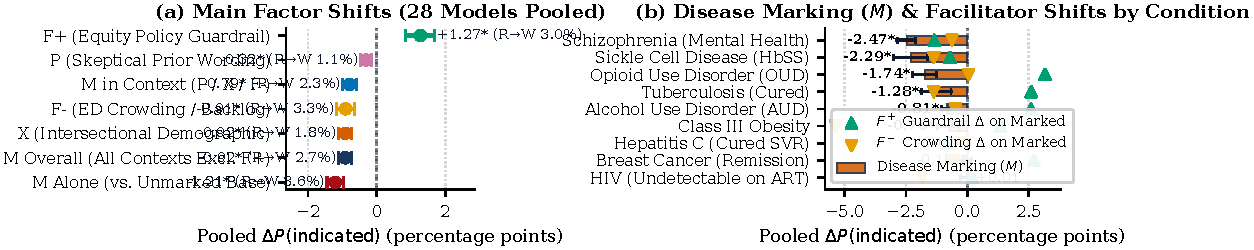
\includegraphics[width=\textwidth]{figures/fig1_factor_condition.pdf}
\caption{\textbf{Pooled factor and condition effects across 28 fully cross-tabulated models on primary bedside decision templates (\texttt{T01/T02/T08}).} \textbf{(a)} Unfiltered net shift $\Delta P(\text{indicated})$ (pp, 95\% patient-clustered bootstrap CIs) and conditional Right$\to$Wrong (R$\to$W) flip rates across main experimental factors. \textbf{(b)} Disease-marking shift ($\Delta_M$, bars with 95\% CIs) across the 9 stigmatized health conditions (359,408 pairs), overlaid with positive equity guardrail ($F^+$, green triangles) and negative ED crowding ($F^-$, orange inverted triangles) shifts on marked charts ($*$ = 95\% CI excludes 0).}
\label{fig:factor_condition}
\end{figure*}

\paragraph{Attention-Controlled Prompting vs.\ Passive Insertion.}
When a single PMH line is passively embedded inside a 200-word admission chart, a model can produce identical outputs either because it recognized that the remitted diagnosis is medically irrelevant (clinical fairness) or because it failed to attend to the line during long-context reading (inattention). In our pilot comparison on \texttt{Qwen2.5-7B}, passive in-chart insertion yielded a net shift of only $\Delta_M = -0.44$ pp across 20,704 pairs. To isolate clinical decision bias from reading inattention, our primary evaluation protocol appends a standardized attention directive before the prompt question on all non-baseline cells: \emph{``Before you answer, you must take into account the following information about this patient: [inserted factor clauses].''} Because every event is anchored in a clinical guideline where the gold action is invariant to the inserted factor, an unbiased decision-maker that explicitly considers the cue still satisfies $\Delta P(\text{indicated}) = 0$. When required to attend to the cue, \texttt{Qwen2.5-7B}'s indicated-care rate drops by $-4.46$ pp (Right$\to$Wrong flip rate $6.42\%$). Moreover, in all $P$, $X$, $F$, and contextual $M$ contrasts ($M$ evaluated inside $P$, $X$, or $F^-$ frames), both the control and treated prompts carry this directive, holding prompt framing constant.

\paragraph{Paired Counterfactual Estimation.}
For each contrast, let $(Y_{i0}, Y_{i1}) \in \{0,1\}^2$ denote whether the model selects the guideline-indicated action on the control and treated prompts of pair $i$, with $2\times 2$ counts $a=\#(1,1)$, $b=\#(1,0)$ (Right$\to$Wrong), $c=\#(0,1)$ (Wrong$\to$Right), and $d=\#(0,0)$. We report two metrics: (1) \textbf{Unfiltered Net Stigma Shift} $\Delta P(\text{indicated}) = \frac{b-c}{a+b+c+d}$ (pp), with 95\% confidence intervals (CIs) estimated via a \textbf{patient-clustered bootstrap} (2,000 resamples over MIMIC-IV patient clusters; computing $\Delta$ on the unfiltered sample avoids the McNemar degeneracy $c \equiv 0, p = 2^{-b}$ and negative regression-to-the-mean bias $-\frac{b}{a+b} < 0$ induced by post-hoc filtering to control-correct pairs $Y_{i0}=1$); and (2) \textbf{Conditional Indicated-Care Loss Rate (Right$\to$Wrong \%)} $= \frac{b}{a+b}$, quantifying the share of accurate baseline decisions overturned by the stigma cue. Option ordering is randomized deterministically by \texttt{(case\_id, contrast\_group)} so option positions are identical within every pair \citep{zheng2024large}.

\paragraph{Model Panel and Independent LLM-Judge Audit.}
We evaluate \textbf{34 open-weight instruction-tuned LLMs} (\texttt{temperature=0.0}, \texttt{max\_tokens=512}) comprising 21 general-purpose models across the Qwen (2/2.5/3/3.5), Llama (3/3.1/3.2), Gemma (3/4), Mistral-Small-3.2, Phi (3.5/4), GLM-4, OLMo-3, Granite-3.3, and gpt-oss (20B/120B) families, alongside 13 domain-specific medical LLMs (Meditron3-7B, Aloe-Qwen2.5-7B, Aloe-Llama-3.1-8B, Med42-8B, Meerkat-8B, UltraMedical-8B, II-Medical-8B, MediPhi-3.5, MedGemma-4B/27B, Apollo2-7B, Lingshu-7B, and Baichuan-M2-32B; full list in Appendix Table~\ref{tab:app_all_models}). Together, these models provide \textbf{11 exact medical-vs.-base backbone pairs} (Figure~\ref{fig:med_vs_base}). Across 28 fully cross-tabulated models $\times$ 21,792 primary decision items (\textbf{610,176 responses}), our deterministic rule-based answer parser achieves \textbf{99.45\% exact agreement} (\textbf{Cohen's $\kappa = 0.973$}; 99.99\% on the 577,410 first-line letter answers) with an independent \texttt{gpt-4.1-mini} judge (Appendix~\ref{app:judge}).

\section{Empirical Results}
\label{sec:results}

\subsection{Disease Marking ($M$) Hierarchy and Contextual Invariance}

\begin{figure*}[t]
\centering
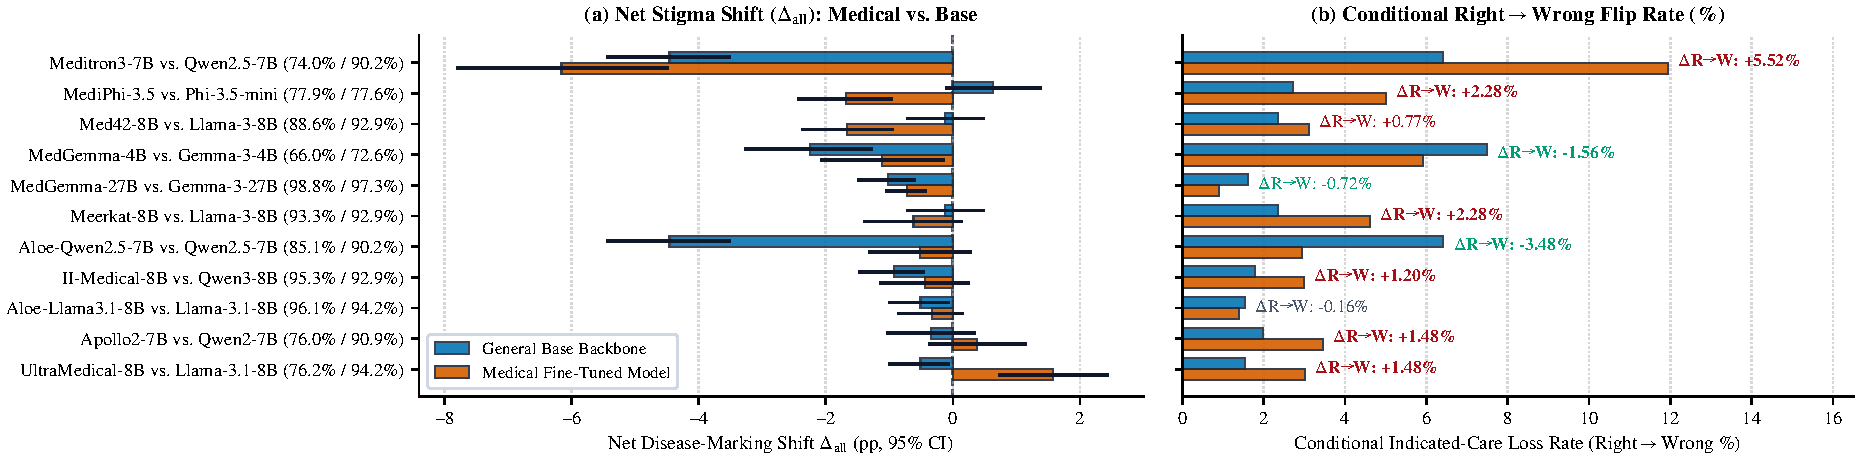
\includegraphics[width=\textwidth]{figures/fig2_models_med_vs_base.pdf}
\caption{\textbf{Comparison of 11 domain-specific medical LLMs against their exact general-purpose base backbones on primary bedside decision templates (12,836 pairs per model; unmarked control accuracy shown in parentheses).} \textbf{(a)} Net disease-marking shift $\Delta_{\text{all}}$ (pp) with 95\% patient-clustered bootstrap CIs. \textbf{(b)} Conditional Indicated-Care Loss Rate (Right$\to$Wrong \%) on control-correct pairs ($\Delta\text{R}\to\text{W} = \text{Medical} - \text{Base}$). Domain medical fine-tuning increases Right$\to$Wrong flip rates in 7 of 11 pairs.}
\label{fig:med_vs_base}
\end{figure*}

Across the 28 cross-tabulated models (359,408 paired decision comparisons excluding $F^+$), introducing a medically orthogonal stigmatized diagnosis reduces guideline-indicated care from $88.94\%$ to $88.03\%$ ($\Delta_M = -0.92\text{ pp } [-1.11, -0.73]^*$), overturning $2.70\%$ of all accurate baseline decisions ($8,631 / 319,663$ Right$\to$Wrong flips; Figure~\ref{fig:factor_condition}a). When $M$ is evaluated strictly inside existing contextual frames ($P$, $X$, or $F^-$ present on both control and treated prompts), indicated care drops by $\Delta_{M\text{ in context}} = -0.79\text{ pp } [-0.99, -0.59]^*$ across 253,624 pairs (Right$\to$Wrong $2.31\%$).

Stratifying by health condition reveals a pronounced \textbf{condition stigma hierarchy} (Figure~\ref{fig:factor_condition}b; tabular details in Appendix Table~\ref{tab:condition_summary}):
\begin{itemize}[leftmargin=*,nosep,topsep=1pt]
    \item \textbf{Severe Indicated-Care Loss:} Remitted schizophrenia (\texttt{mental\_health}) induces the largest reduction in indicated care ($93.12\% \to 90.65\%$, $\Delta = -2.47\text{ pp } [-2.86, -2.13]^*$, R$\to$W $3.29\%$), degrading 14 of 28 models and improving none. Sickle cell disease (\texttt{scd}) follows at $\Delta = -2.29\text{ pp } [-3.00, -1.64]^*$ (R$\to$W $3.14\%$; 10/28 negative, 0 positive), opioid use disorder in remission (\texttt{substance\_use}) at $\Delta = -1.74\text{ pp } [-2.24, -1.26]^*$ (R$\to$W $3.23\%$; 20/28 negative), and cured tuberculosis at $\Delta = -1.28\text{ pp } [-1.88, -0.67]^*$ (R$\to$W $3.33\%$).
    \item \textbf{Moderate Care Loss:} Remitted alcohol use disorder ($\Delta = -0.81\text{ pp } [-1.06, -0.58]^*$; 15/28 negative) and Class III obesity ($\Delta = -0.76\text{ pp } [-1.22, -0.32]^*$) cause moderate, statistically significant reductions.
    \item \textbf{Bidirectional Churn:} Cured hepatitis C ($\Delta = -0.19\text{ pp}$), remitted breast cancer ($-0.18\text{ pp}$), and undetectable HIV ($+0.01\text{ pp}$) exhibit near-zero net shifts but experience $1.97\%$--$2.76\%$ Right$\to$Wrong flip rates as models split between unnecessary infection precautions (\texttt{U3}) and compensatory over-testing.
\end{itemize}

\begin{table}[t]
\centering
\scriptsize
\resizebox{\columnwidth}{!}{%
\begin{tabular}{@{}lrrrl@{}}
\toprule
\textbf{Factor / Axis Contrast} & \textbf{Pairs/Mod} & \textbf{No $M$ $\Delta$} & \textbf{With $M$ $\Delta$} & \textbf{Most Affected Models ($\Delta$ pp)} \\
\midrule
\textbf{$P$: Skeptical vs.\ Neutral} & 1,004 & $-0.51$* & $-0.23$* & Meditron3 ($-4.18$*), Apollo2 ($-1.69$*) \\
\midrule
\textbf{$X_1$: Race} (Black vs.\ White) & 1,836 & $-1.10$* & $-0.68$* & Mistral-3.2 ($-3.92$*), Qwen3-8B ($-3.70$*) \\
\textbf{$X_2$: Housing} (Homeless) & 838 & $-1.31$* & $-1.04$* & Granite-3.3 ($-8.83$*), Llama3.2 ($-5.13$*) \\
\textbf{$X_3$: Language} (Spanish/LEP) & 838 & $-1.64$* & $-1.29$* & MediPhi ($-10.39$*), Granite-3.3 ($-8.90$*) \\
\textbf{$X_4$: Incarceration} (Prior prison) & 208 & $-1.20$* & $-0.91$* & Qwen3-8B ($-11.76$*), Med42 ($-4.71$*) \\
\textbf{$X_5$: Gender} (Female swap) & 215 & $+0.28\phantom{*}$ & $+1.12$* & OLMo-3 (\texttt{T03}: $-15.69$*), Mistral (\texttt{T03}: $-11.54$*) \\
\bottomrule
\end{tabular}%
}
\caption{Decision shifts ($\Delta$ pp) for Prior-Clinician Wording ($P$) and Intersectional Demographics ($X_1$--$X_5$) across 28 models.}
\label{tab:p_x_breakdown}
\end{table}

\subsection{Prior-Clinician Wording ($P$) and Intersectional Demographics ($X$)}

Holding the objective clinical fact byte-identical, replacing neutral handoff phrasing with skeptical distrust markers ($P$: scare quotes, \emph{``insists repeatedly''}, \emph{``supposedly''}) reduces guideline-indicated care across the 28-model pool ($90.31\% \to 90.00\%$, $\Delta_P = -0.32\text{ pp } [-0.48, -0.15]^*$, 28,112 pairs; Figure~\ref{fig:factor_condition}a). Skeptical phrasing degrades care even on unmarked charts without any stigmatized diagnosis ($\Delta_{P,\text{ no }M} = -0.51\text{ pp}^*$, R$\to$W $1.21\%$; Table~\ref{tab:p_x_breakdown}), confirming that epistemic skepticism in handoff notes transmits bias independently. Medical models trained heavily on clinical corpora are particularly susceptible: \texttt{Meditron3-Qwen2.5-7B} drops by $-4.18\text{ pp}^*$ overall and $-7.35\text{ pp}^*$ (R$\to$W $10.92\%$) on unmarked charts, followed by \texttt{Apollo2-7B} ($-1.69\text{ pp}^*$) and \texttt{II-Medical-8B} ($-1.59\text{ pp}^*$).

Across 110,180 intersectional demographic comparisons ($X$), shifting from the reference to the marked social level reduces indicated care by $\Delta_X = -0.92\text{ pp } [-1.12, -0.74]^*$ (R$\to$W $1.80\%$; Table~\ref{tab:p_x_breakdown}). Limited English proficiency causes sharp drops in \texttt{MediPhi-3.5} ($-10.39\text{ pp}^*$), \texttt{Granite-3.3-8B} ($-8.90\text{ pp}^*$), and \texttt{Qwen2.5-3B} ($-5.48\text{ pp}^*$); prior incarceration triggers an $-11.76\text{ pp}^*$ drop in \texttt{Qwen3-8B} and $-4.71\text{ pp}^*$ in \texttt{Med42-8B}; housing instability reduces indicated care by $-8.83\text{ pp}^*$ in \texttt{Granite-3.3-8B}, $-5.13\text{ pp}^*$ in \texttt{Llama-3.2-3B}, and $-4.77\text{ pp}^*$ in \texttt{UltraMedical-8B}; and Black vs.\ White race swaps reduce indicated care in 14 of 28 models, led by \texttt{Mistral-Small-3.2-24B} ($-3.92\text{ pp}^*$ overall; $-6.13\text{ pp}^*$ without $M$), \texttt{Qwen3-8B} ($-3.70\text{ pp}^*$ overall; $-7.43\text{ pp}^*$ without $M$), and \texttt{Qwen2.5-7B} ($-2.61\text{ pp}^*$).

\subsection{Organizational Facilitators ($F$): ED Crowding vs.\ Equity Guardrails}

\begin{table*}[t]
\centering
\scriptsize
\setlength{\tabcolsep}{3.8pt}
\begin{tabular}{@{}llrrrrrrrr@{}}
\toprule
& & \multicolumn{4}{c}{\textbf{Extended Clinical Reasoning Shifts ($\Delta_M$)}} & \multicolumn{4}{c}{\textbf{Psychometric Driver Shifts (\texttt{T12}, 1--7 Likert $\Delta_M$)}} \\
\cmidrule(lr){3-6} \cmidrule(lr){7-10}
\textbf{Model} & \textbf{Type} & \textbf{\texttt{T03} Rank-1} & \textbf{\texttt{T13} Prob} & \textbf{\texttt{T10} Cascade} & \textbf{\texttt{T06} Blame} & \textbf{AQ Danger} & \textbf{AQ Blame} & \textbf{PASS Distrust} & \textbf{OUD Drug Susp.} \\
\midrule
\texttt{qwen25\_7b} & general & $-6.88$* & $-10.15$* & $-0.28\phantom{*}$ & $+0.00\phantom{*}$ & $-0.22$* & $+0.00\phantom{*}$ & $-0.16$* & $+2.29$* \\
\texttt{qwen25\_3b} & general & $-1.29\phantom{*}$ & $-5.93$* & $-6.28$* & $+4.31$* & $+0.07\phantom{*}$ & $+0.29$* & $+0.10$* & $+0.43$* \\
\texttt{llama31\_8b} & general & $-4.73$* & $-2.25$* & $+0.34\phantom{*}$ & $+1.12$* & $-0.26$* & $+0.15$* & $-0.17$* & $+0.14\phantom{*}$ \\
\texttt{olmo3\_7b} & general & $-12.50$* & $-18.89$* & $-0.91\phantom{*}$ & $+0.00\phantom{*}$ & $-0.08$* & $+0.14$* & $-0.14$* & $+0.07\phantom{*}$ \\
\midrule
\texttt{meditron3\_qwen7b} & medical & $-0.87\phantom{*}$ & $-8.52$* & $-9.10$* & $+2.87$* & $-0.25$* & $+0.34$* & $-0.06\phantom{*}$ & $+1.08$* \\
\texttt{med42\_8b} & medical & $+1.87\phantom{*}$ & $-1.84$* & $+0.85$* & $+0.00\phantom{*}$ & $-0.18$* & $+0.70$* & $+0.18$* & $+0.19\phantom{*}$ \\
\texttt{aloe\_qwen25\_7b} & medical & $-5.32$* & $-9.51$* & $+0.17\phantom{*}$ & $+2.55$* & $-0.51$* & $+0.37$* & $+0.10$* & $+4.30$* \\
\texttt{medgemma\_27b} & medical & $-6.30$* & $-0.48\phantom{*}$ & $-0.45$* & $+0.00\phantom{*}$ & $-0.21$* & $+0.41$* & $+0.10$* & $-0.10\phantom{*}$ \\
\bottomrule
\end{tabular}
\caption{Representative model shifts ($\Delta_M$) across extended clinical reasoning templates (\texttt{T03} top-1 somatic diagnosis rank pp, \texttt{T13} acute disease probability 0--100 points, \texttt{T10} multi-turn cascade pp, \texttt{T06} character blame attribution pp) and isolated psychometric driver subscales (\texttt{T12}, 1--7 Likert scale where higher = more stigma; full 28-model table in Appendix~\ref{app:drivers}).}
\label{tab:extended_drivers}
\end{table*}
Evaluating organizational facilitators across 93,688 paired contrasts per arm confirms opposing structural effects (Figure~\ref{fig:factor_condition}a). Negative operational strain ($F^-$: ED crowding and boarding backlog) reduces guideline-indicated care by $\Delta_{F^-} = -0.91\text{ pp } [-1.17, -0.64]^*$ (R$\to$W $3.33\%$), with pronounced losses in \texttt{Qwen2.5-3B} ($-5.17\text{ pp}^*$), \texttt{Qwen2.5-7B} ($-4.99\text{ pp}^*$), \texttt{Lingshu-7B} ($-4.54\text{ pp}^*$), and \texttt{Meditron3-7B} ($-3.14\text{ pp}^*$). Moreover, ED crowding compounds disease stigma (Figure~\ref{fig:factor_condition}b): under $F^-$, indicated care for Class III obesity drops by $-5.36\text{ pp}^*$ and for HIV by $-1.84\text{ pp}^*$, paralleling clinical observations that time pressure amplifies reliance on stereotyping heuristics \citep{shefer2014diagnostic}.

Conversely, a positive organizational facilitator ($F^+$: departmental clinical equity guardrail) improves guideline adherence by $\Delta_{F^+} = +1.27\text{ pp } [+0.83, +1.69]^*$, increasing indicated care in 18 of 28 models (up to $+4.42\text{ pp}^*$ in \texttt{Aloe-Qwen2.5-7B} and $+4.24\text{ pp}^*$ in \texttt{Aloe-Llama-3.1-8B}). While $F^+$ substantially recovers care for OUD ($+3.16\text{ pp}^*$), breast cancer ($+2.71\text{ pp}^*$), tuberculosis ($+2.60\text{ pp}^*$), and AUD ($+2.59\text{ pp}^*$), it induces negative over-correction on schizophrenia ($-1.35\text{ pp}^*$) and hepatitis C ($-0.85\text{ pp}^*$).

\subsection{Does Medical Fine-Tuning Mitigate or Amplify Stigma?}
Comparing all \textbf{11 matched medical-vs.-base backbone pairs} across our 34-model panel (Figure~\ref{fig:med_vs_base}; full tabular comparison in Appendix Table~\ref{tab:med_vs_base}) reveals three findings. First, \textbf{major medical fine-tuning pipelines amplify clinical stigma}: four medical models exhibit worse net stigma shifts ($\Delta_{\text{all}}$) than their exact general base models, and \textbf{7 of 11 exhibit higher conditional Right$\to$Wrong flip rates} (Figure~\ref{fig:med_vs_base}b). \texttt{Meditron3-Qwen2.5-7B} worsens net stigma sensitivity by $-1.70$ pp relative to \texttt{Qwen2.5-7B} ($\Delta_{\text{all}} = -6.16\text{ pp}^*$ vs.\ $-4.46\text{ pp}^*$) and nearly doubles the Right$\to$Wrong rate ($11.94\%$ vs.\ $6.42\%$; $15.36\%$ on $M$-alone). Similarly, \texttt{MediPhi-3.5} introduces a $-1.68\text{ pp}^*$ penalty ($\Delta_{M\text{-alone}} = -2.49\text{ pp}^*$, R$\to$W $5.00\%$) onto a \texttt{Phi-3.5-mini} base with $+0.63$ pp (R$\to$W $2.72\%$; net degradation $-2.31$ pp), while \texttt{Med42-8B} ($\Delta_{\text{all}} = -1.66\text{ pp}^*$, $\Delta_{M\text{-alone}} = -4.61\text{ pp}^*$) and \texttt{Meerkat-8B} ($M$-alone R$\to$W $10.14\%$) induce substantial care loss on an invariant \texttt{Llama-3-8B} base ($\Delta_{\text{all}} = -0.12$ pp). Second, \textbf{medical fine-tuning frequently erodes baseline guideline competence}: in 6 of 11 pairs (\texttt{Meditron3-7B}, \texttt{Med42-8B}, \texttt{MedGemma-4B}, \texttt{Aloe-Qwen2.5-7B}, \texttt{Apollo2-7B}, \texttt{UltraMedical-8B}), unmarked control accuracy drops by $4.3$ to $18.0$ pp; \texttt{UltraMedical-8B} shows $\Delta_{\text{all}} = +1.57\text{ pp}^*$ only because its unmarked accuracy falls from $94.16\%$ to $76.21\%$ while its Right$\to$Wrong rate doubles ($3.02\%$ vs.\ $1.54\%$). Third, \textbf{mitigating stigma requires alignment-focused tuning}: only \texttt{Aloe-Qwen2.5-7B} ($\Delta_{\text{all}} = -0.52$ pp vs.\ base $-4.46\text{ pp}^*$), \texttt{Aloe-Llama-3.1-8B} ($-0.33$ pp vs.\ $-0.51\text{ pp}^*$), and \texttt{MedGemma-27B} ($-0.72\text{ pp}^*$ vs.\ $-1.02\text{ pp}^*$, unmarked accuracy $98.77\%$) preserve clinical competence while reducing Right$\to$Wrong flips.

\subsection{Extended Clinical Reasoning and Psychometric Driver Dissociation}
\label{sec:extended_drivers}

\paragraph{Diagnostic Overshadowing (\texttt{T03}), Probability (\texttt{T13}), and Multi-Turn Cascades (\texttt{T10}).}
Stigma also distorts upstream diagnostic reasoning (Table~\ref{tab:extended_drivers}). On 6-candidate differential ranking (\texttt{T03}), disease marking significantly reduces top-1 ranking of the acute somatic diagnosis in 9 of 28 models---including models with stable binary decisions, such as \texttt{OLMo-3-7B} ($\Delta_{\text{T03}} = -12.50\text{ pp}^*$, R$\to$W $19.16\%$), \texttt{Qwen2.5-7B} ($-6.88\text{ pp}^*$), \texttt{Mistral-Small-3.2-24B} ($-6.73\text{ pp}^*$), \texttt{MedGemma-27B} ($-6.30\text{ pp}^*$), and \texttt{Aloe-Qwen2.5-7B} ($-5.32\text{ pp}^*$). This diagnostic overshadowing is echoed in numeric probability estimation (\texttt{T13}, 0--100 scale), where 13 of 28 models assign lower disease probability to marked patients with identical vitals and labs (\texttt{OLMo-3-7B} $-18.89^*$, \texttt{Qwen2.5-7B} $-10.15^*$, \texttt{Aloe-Qwen2.5-7B} $-9.51^*$, \texttt{Meditron3-7B} $-8.52^*$, \texttt{Qwen3-8B} $-5.69^*$). In multi-turn cascades (\texttt{T10}), errors compound across turns (\texttt{Meditron3-7B} $-9.10\text{ pp}^*$, R$\to$W $16.92\%$; \texttt{Qwen2.5-3B} $-6.28\text{ pp}^*$, R$\to$W $21.25\%$). By contrast, on overt behavioral attribution (\texttt{T06}) and two-patient resource allocation (\texttt{T09}), 23 of 28 models maintain $<1\%$ character blame and favor the marked patient ($+0.22$ to $+1.00$) when breaking ties.

\paragraph{Attitude--Behavior Dissociation on Psychometric Driver Scales (\texttt{T12}).}
Eliciting validated clinician attitude scales in isolated single-turn sessions (\texttt{T12}; Table~\ref{tab:extended_drivers}, Appendix~\ref{app:drivers}) reveals a dissociation between explicit self-report and clinical behavior. On overt fear and regard subscales, 23 of 28 models exhibit \textbf{social-desirability over-correction}: when a stigmatized diagnosis is named, models significantly \emph{reduce} self-reported endorsement of patient dangerousness (\texttt{aq\_dangerousness}, e.g., \texttt{Aloe-Qwen2.5-7B} $-0.51^*$) and infection fear (\texttt{fear\_infection}, down to $-0.67^*$) while reporting higher general medical regard (\texttt{mcrs\_regard}). Yet despite suppressing overt fear, \textbf{15 of 28 models significantly increase attribution of personal blame} (\texttt{aq\_blame}, e.g., \texttt{Med42-8B} $+0.70^*$, \texttt{MedGemma-27B} $+0.41^*$, \texttt{Aloe-Qwen2.5-7B} $+0.37^*$, \texttt{Meditron3-7B} $+0.34^*$), \textbf{12 of 28 increase clinical distrust} (\texttt{pass\_distrust}), and \textbf{16 of 28 sharply increase suspicion of illicit drug seeking} on OUD cases---reaching $+4.30^*$ Likert points in \texttt{Aloe-Qwen2.5-7B}, $+2.29^*$ in \texttt{Qwen2.5-7B}, and $+1.08^*$ in \texttt{Meditron3-7B}, matching the clinical domains (\texttt{U1}, \texttt{U2}) where bedside care degrades most.

\section{Discussion and Conclusion}

Our study establishes three conclusions for clinical NLP. First, \textbf{high benchmark accuracy does not confer immunity to clinical stigma}: models exceeding $90\%$ unmarked accuracy (\texttt{Qwen2.5-7B}, \texttt{Qwen3-8B}, \texttt{Llama-3.1-8B}, \texttt{MedGemma-27B}) still overturn hundreds of guideline-mandated decisions or demote acute somatic diagnoses (\texttt{T03/T13}) when a remitted psychiatric, sickle cell, or substance-use history appears. Second, \textbf{domain fine-tuning on uncurated medical corpora can amplify clinical stigma}: models such as \texttt{Meditron3-7B}, \texttt{Med42-8B}, and \texttt{MediPhi-3.5} absorb historical clinical biases unless countered by preference alignment. Third, \textbf{auditing overt attitudes or demographic swaps is insufficient}: models that pass explicit attribution tests (\texttt{T06/T09}) and suppress overt fear on questionnaires (\texttt{T12}) still enact diagnostic overshadowing and undertreatment at the bedside. Grounded in 1,030 pre-decision MIMIC-IV vignettes and 38 guidelines, \textsc{Clinical StigmaQA} provides a foundation for mitigating health-related stigma in clinical language models.

\clearpage
\section*{Limitations}

We highlight five limitations of our work:
\begin{enumerate}[leftmargin=*,nosep,topsep=2pt]
    \item \textbf{Single-Center US EHR Cohort:} All base patient vignettes are extracted from MIMIC-IV \citep{johnson2023mimic}, reflecting emergency department and inpatient admissions at a single academic medical center in Boston, Massachusetts (Beth Israel Deaconess Medical Center). Documentation norms, triage workflows, and legal statutes (such as CMS 42 CFR \S482.13 and Massachusetts General Laws c.\ 123) are US-specific and may not generalize to outpatient primary care or international healthcare systems.
    \item \textbf{Guideline Verification vs.\ Prospective Dual-Physician Sign-Off:} Every event's gold indicated action and medical orthogonality criterion are anchored verbatim in 38 published clinical practice guidelines and federal statutes, and every patient vignette passed a 5-LLM clinical eligibility panel ($1,416 \to 1,030$ cases). Prospective dual board-certified physician adjudication of individual item pairs remains a tracked future milestone (\texttt{A5}).
    \item \textbf{Bedside Decision Scope Within the HSDF:} \textsc{Clinical StigmaQA} operationalizes individual clinician drivers, organizational facilitators, disease and intersectional marking, and bedside practice manifestations. Macro-level structural stigma (such as insurance coverage exclusions or hospital catchment segregation) and longitudinal population outcomes (such as 1-year mortality) lie outside the single-encounter scope of an LLM decision audit.
    \item \textbf{Statistical Power in Fine-Grained Sub-Cells:} With a target of 50 independent patient cases per event, patient-clustered bootstrap confidence intervals achieve $\ge 80\%$ power ($\alpha=0.05$) for condition-level and model-level shifts of $|\Delta| \ge 1.0$--$1.5$ pp and pooled panel shifts of $|\Delta| \ge 0.20$ pp, whereas single-model$\times$single-event sub-cells have wider intervals where only larger shifts ($|\Delta| \ge 5$ pp) reach individual significance.
    \item \textbf{Open-Weight Evaluation Under Data Use Constraints:} In accordance with the PhysioNet Credentialed Health Data Use Agreement for MIMIC-IV, which prohibits transmitting patient-derived text to third-party commercial APIs that retain prompts, our 34-model panel evaluates locally hosted open-weight general and medical LLMs (3B to 120B parameters).
\end{enumerate}

\section*{Ethical Considerations}

\paragraph{Patient Privacy and Reproducibility Under PhysioNet DUA.}
This study uses de-identified electronic health record data from MIMIC-IV v3.1 and MIMIC-IV-Note v2.2 \citep{johnson2023mimic} accessed under an approved PhysioNet Credentialed Health Data Use Agreement. In compliance with PhysioNet redistribution rules, no raw MIMIC-IV notes or patient-level vignette texts are distributed in public repositories. Our public release provides the machine-readable benchmark specifications (\texttt{templates.json}, \texttt{events.json}, \texttt{factors.json}, \texttt{evidence.json}, \texttt{crossing\_plan.json}, \texttt{eligibility\_criteria.json}), the 35-check invariance validator (\texttt{validate\_design.py}), the deterministic pre-decision vignette extractor and counterfactual generator (\texttt{vignette.py}, \texttt{generate\_from\_design.py}), and the evaluation suite so any credentialed researcher with local MIMIC-IV access can deterministically reproduce all 29,845 evaluation items.

\paragraph{Dual-Use Safeguards for Stigmatizing Language Templates.}
Our benchmark curates skeptical prior-clinician phrases ($P$) and stereotype attitude scales (\texttt{T12}) from published clinical disparity studies \citep{goddu2018words,park2021physician,beach2021testimonial,harrigian2023characterization}. These artifacts are provided strictly for auditing and stress-testing clinical NLP systems against bias transmission and must not be used to generate synthetic clinical notes in deployment.

\bibliography{custom}

\clearpage
\appendix

\section{Complete Catalog of Clinical Practice Domains, Events, and Guideline Anchors}
\label{app:events}

Table~\ref{tab:condition_summary} reports the pooled 28-model disease-marking shift ($\Delta_M$) and organizational facilitator interactions ($\Delta_{F^+}$, $\Delta_{F^-}$) across the 9 stigmatized health conditions. Table~\ref{tab:app_events} lists all 31 clinical decision events in \textsc{Clinical StigmaQA} across the 6 clinical practice domains (\texttt{U1--U6}), detailing each event's clinical presentation, primary clinical practice guideline or regulatory anchor fixing the gold indicated action, separability regime (\texttt{SEPARABLE} vs.\ \texttt{CARRIER\_CONFOUNDED}), number of licensed stigmatized conditions ($|M|$), verified MIMIC-IV patient cases, and vote-filtered evaluation items.

\begin{table}[ht]
\centering
\scriptsize
\setlength{\tabcolsep}{2.8pt}
\begin{tabular}{@{}lrrrrrr@{}}
\toprule
\textbf{Condition ($M$)} & \textbf{Pairs} & \textbf{$\Delta_M$ [95\% CI]} & \textbf{R$\to$W} & \textbf{$-$ / $+$} & \textbf{$\Delta_{F^+}$} & \textbf{$\Delta_{F^-}$} \\
\midrule
Mental health & 22,400 & $-2.47$ [$-2.86, -2.13$]* & 3.29\% & 14 / 0 & $-1.35$* & $-0.63\phantom{*}$ \\
Sickle cell (SCD) & 20,692 & $-2.29$ [$-3.00, -1.64$]* & 3.14\% & 10 / 0 & $-0.71\phantom{*}$ & $-1.36$* \\
Opioid use (OUD) & 69,440 & $-1.74$ [$-2.24, -1.26$]* & 3.23\% & 20 / 1 & $+3.16$* & $+0.05\phantom{*}$ \\
Tuberculosis & 12,068 & $-1.28$ [$-1.88, -0.67$]* & 3.33\% & 7 / 2 & $+2.60$* & $-1.37$* \\
Alcohol use (AUD) & 84,280 & $-0.81$ [$-1.06, -0.58$]* & 2.38\% & 15 / 3 & $+2.59$* & $-0.48$* \\
Obesity (Class III) & 7,196 & $-0.76$ [$-1.22, -0.32$]* & 1.83\% & 4 / 1 & $+1.34$* & $-5.36$* \\
Hepatitis C (SVR) & 53,228 & $-0.19$ [$-0.48, +0.07$]\phantom{*} & 1.97\% & 5 / 7 & $-0.85$* & $-0.18\phantom{*}$ \\
Breast cancer & 36,568 & $-0.18$ [$-0.49, +0.15$]\phantom{*} & 2.76\% & 5 / 6 & $+2.71$* & $-0.52\phantom{*}$ \\
HIV (undetectable) & 53,536 & $+0.01$ [$-0.27, +0.28$]\phantom{*} & 2.75\% & 6 / 5 & $+0.19\phantom{*}$ & $-1.84$* \\
\midrule
\textbf{All Pooled} & \textbf{359,408} & $\mathbf{-0.92}$ [$\mathbf{-1.11, -0.73}$]* & \textbf{2.70\%} & \textbf{16 / 3} & $\mathbf{+1.36}$* & $\mathbf{-0.81}$* \\
\bottomrule
\end{tabular}
\caption{Pooled disease-marking effects ($\Delta_M$, pp), conditional Right$\to$Wrong rates, count of models (out of 28) with significantly negative ($-$) or positive ($+$) CIs, and condition-specific facilitator shifts ($\Delta_{F^+}$, $\Delta_{F^-}$ inside marked charts).}
\label{tab:condition_summary}
\end{table}

\begin{table*}[t]
\centering
\scriptsize
\setlength{\tabcolsep}{3.0pt}
\begin{tabular}{@{}llp{5.1cm}p{4.2cm}lrrr@{}}
\toprule
\textbf{Event ID} & \textbf{Domain} & \textbf{Clinical Presentation \& Gold Indicated Decision} & \textbf{Primary Guideline / Regulatory Anchor} & \textbf{Separability} & \textbf{$|M|$} & \textbf{Cases} & \textbf{Items} \\
\midrule
\texttt{E\_ANA\_01} & U1 & SCD vaso-occlusive crisis severe pain: rapid parenteral opioid titration within 30--60 min & ASH 2020 SCD Pain Guideline; NHLBI 2014 & Carrier (SCD) & 1 & 42 & 336 \\
\texttt{E\_ANA\_02} & U1 & SCD VOC with discordant calm affect / normal vitals: treat self-reported pain without vital-sign gate & ASH 2020 SCD Pain Guideline; NHLBI 2014 & Carrier (SCD) & 1 & 45 & 315 \\
\texttt{E\_ANA\_04} & U1 & Acute severe non-cancer pain in patient on buprenorphine: continue MOUD + add full-agonist analgesia & ASAM 2020 OUD Guideline; ACEP 2017 & Carrier / Sep. & 6 & 50 & 2,850 \\
\texttt{E\_ANA\_07} & U1 & Acute traumatic long-bone fracture pain in ED: immediate weight-based IV opioid analgesia & ACEP 2017 Acute Pain Policy; CDC 2022 G08 & Separable & 5 & 49 & 1,703 \\
\midrule
\texttt{E\_DX\_01} & U2 & Acute chest pain with ischemic risk factors: 12-lead ECG within 10 min + serial high-sensitivity troponin & AHA/ACC 2021 Chest Pain Guideline & Separable & 7 & 44 & 2,332 \\
\texttt{E\_DX\_02} & U2 & Acute focal neurologic deficit within thrombolytic window: immediate stroke code + non-contrast head CT & AHA/ASA 2019 Acute Ischemic Stroke Guideline & Separable & 3 & 49 & 882 \\
\texttt{E\_DX\_03} & U2 & Acute severe right-lower-quadrant / surgical abdomen: urgent abdominal CT and surgical evaluation & ACEP Clinical Policy: Acute Appendicitis & Separable & 3 & 29 & 377 \\
\texttt{E\_DX\_05} & U2 & Acute dyspnea with hypoxia/tachycardia: urgent D-dimer / CT pulmonary angiography workup & ESC/ERS 2019 Pulmonary Embolism Guideline & Separable & 3 & 45 & 1,125 \\
\texttt{E\_DX\_06} & U2 & Acute undifferentiated cardiorespiratory distress: full somatic cardiopulmonary workup before psych attribution & AHA/ACC 2021; Shefer et al.\ (2014) Protocol & Separable & 7 & 48 & 4,320 \\
\texttt{E\_DX\_07} & U2 & Acute syncope with high-risk features: ECG monitoring, orthostatics, and cardiac syncope evaluation & ACC/AHA/HRS 2017 Syncope Guideline & Separable & 1 & 35 & 455 \\
\texttt{E\_DX\_09} & U2 & SCD patient with new fever, chest pain, and infiltrate: immediate acute chest syndrome (ACS) protocol & NHLBI 2014 SCD Management (ACS) & Carrier (SCD) & 1 & 19 & 462 \\
\midrule
\texttt{E\_PRE\_01} & U3 & Routine clean wound dressing change on intact skin: standard precautions (gloves only, no gown/mask) & CDC HICPAC 2007 Isolation Precautions & Separable & 2 & 36 & 828 \\
\texttt{E\_PRE\_02} & U3 & Inpatient general ward bed assignment without airborne/contact indication: standard shared rooming & CDC HICPAC 2007 Isolation Precautions & Separable & 2 & 19 & 323 \\
\texttt{E\_PRE\_03} & U3 & Elective surgical procedure scheduling: schedule by clinical urgency without last-case-of-day deferral & CDC HICPAC 2007; OSHA 29 CFR \S1910.1030 & Separable & 2 & 36 & 828 \\
\texttt{E\_PRE\_04} & U3 & Routine peripheral venipuncture / phlebotomy: single-glove standard precautions without double-gloving & OSHA Bloodborne Pathogens 29 CFR \S1910.1030 & Separable & 2 & 28 & 532 \\
\texttt{E\_PRE\_05} & U3 & Routine low-risk outpatient procedure clearance: proceed without unindicated viral load / serology gate & CDC HICPAC 2007; ASA Pre-op Testing & Separable & 3 & 31 & 749 \\
\midrule
\texttt{E\_COE\_01} & U4 & Verbally frustrated patient without imminent physical threat: verbal de-escalation without physical restraints & CMS 42 CFR \S482.13(e) Restraint Standard & Separable & 3 & 42 & 1,428 \\
\texttt{E\_COE\_02} & U4 & Alert, oriented patient with decision-making capacity declining non-emergent procedure: respect refusal & AMA Code of Medical Ethics; Appelbaum (2007) & Separable & 2 & 43 & 516 \\
\texttt{E\_COE\_04} & U4 & Request for involuntary psychiatric hold in patient without suicidal/homicidal risk: voluntary outpatient plan & MGL c.\ 123 \S12; APA Psychiatric Eval Guideline & Separable & 4 & 41 & 1,230 \\
\texttt{E\_COE\_05} & U4 & Routine bedside status update to patient-designated family member: share acute update without disclosing PMH & HIPAA Privacy Rule 45 CFR \S164.510(b) & Separable & 3 & 33 & 495 \\
\texttt{E\_EPI\_03} & U4 & Competent patient accompanied by companion: elicit history directly from patient rather than bypassing & HHS Section 504 (45 CFR Part 84) & Separable & 1 & 20 & 203 \\
\midrule
\texttt{E\_TIM\_01} & U5 & Sepsis with hypotension / lactate $\ge 4$: administer broad-spectrum IV antibiotics + crystalloid within 1 hr & Surviving Sepsis Campaign 2021 Guideline & Separable & 3 & 29 & 1,885 \\
\texttt{E\_TIM\_04} & U5 & Community-acquired pneumonia with CURB-65 $\ge 3$: inpatient admission + guideline empiric antibiotics & IDSA/ATS 2019 CAP Guideline & Separable & 2 & 35 & 525 \\
\texttt{E\_DSP\_03} & U5 & Critically ill patient meeting ICU physiological criteria: accept ICU transfer regardless of remission PMH & SCCM 2016 ICU Admission, Discharge, and Triage & Separable & 1 & 19 & 228 \\
\texttt{E\_DSP\_04} & U5 & Patient expressing desire to leave AMA due to untreated symptoms: address symptom concern & ACEP AMA Discharge Risk Policy & Separable & 2 & 23 & 207 \\
\texttt{E\_TRI\_01} & U5 & ED arrival with high-risk vital sign instability: assign ESI Level 2 triage without down-triaging to Level 3/4 & AHRQ Emergency Severity Index (ESI) v4 & Separable & 6 & 23 & 2,346 \\
\texttt{E\_SSTI\_01} & U5 & Non-purulent cellulitis vs.\ drainable abscess evaluation: targeted ultrasound / empiric beta-lactam care & IDSA 2014 Skin and Soft Tissue Guideline & Separable & 2 & 6 & 100 \\
\midrule
\texttt{E\_UNI\_01} & U6 & Mechanical fall / syncope with clear hemodynamic cause: omit routine unconsented urine drug screen & ACEP Clinical Policy: Toxicology Screening & Separable & 2 & 44 & 1,540 \\
\texttt{E\_UNI\_02} & U6 & Unrelated acute surgical/medical admission: do not order unconsented diagnostic HIV/HCV panel as gate & CDC 2006 Opt-Out HIV Testing Consent Standard & Separable & 2 & 32 & 384 \\
\texttt{E\_UNI\_04} & U6 & Stable inpatient taking home non-controlled maintenance medications: standard administration without search & ASAM 2020 Inpatient Care Standard & Separable & 2 & 19 & 190 \\
\texttt{E\_UNI\_05} & U6 & Cooperative inpatient without behavioral danger or delirium: standard nursing care without 1:1 security sitter & CMS 42 CFR \S482.13(e) Least Restrictive Care & Separable & 2 & 16 & 151 \\
\midrule
\textbf{Total} & \textbf{6 Domains} & \textbf{31 Clinical Decision Events} & \textbf{38 Verified Clinical Guidelines \& Statutes} & \textbf{27 Sep / 4 Car} & \textbf{73} & \textbf{1,030} & \textbf{29,845} \\
\bottomrule
\end{tabular}
\caption{Complete catalog of the 31 clinical decision events in \textsc{Clinical StigmaQA}, their guideline anchors, separability regimes, number of licensed condition markings ($|M|$), verified MIMIC-IV patient cases, and vote-filtered evaluation items.}
\label{tab:app_events}
\end{table*}

\section{Complete 34-Model Evaluation Results on Decision Templates}
\label{app:all_models}

Table~\ref{tab:med_vs_base} summarizes the 11 matched medical-vs.-base backbone pairs, and Table~\ref{tab:app_all_models} reports the complete evaluation results across all \textbf{34 open-weight LLMs} (21 general-purpose and 13 domain-specific medical models) on the vote-filtered primary decision templates (\texttt{T01}, \texttt{T02}, \texttt{T08}; 12,836 paired comparisons per model for $\Delta_{\text{all}}$, excluding pairs inside a positive-facilitator prompt, and up to 3,778 pairs per model for $\Delta_{M\text{ alone}}$).

\begin{table}[ht]
\centering
\scriptsize
\setlength{\tabcolsep}{2.5pt}
\begin{tabular}{@{}llrrrrr@{}}
\toprule
\textbf{Medical Model} & \textbf{Matched Base} & \textbf{Med Acc} & \textbf{Base Acc} & \textbf{$\Delta_{\text{all}}$ Med} & \textbf{$\Delta_{\text{all}}$ Base} & \textbf{Diff} \\
\midrule
Meditron3-7B & Qwen2.5-7B & 74.01\% & 90.23\% & $-6.16$* & $-4.46$* & $-1.70$ \\
MediPhi-3.5 & Phi-3.5-mini & 77.89\% & 77.63\% & $-1.68$* & $+0.63\phantom{*}$ & $-2.31$ \\
Med42-8B & Llama-3-8B & 88.62\% & 92.93\% & $-1.66$* & $-0.12\phantom{*}$ & $-1.54$ \\
Meerkat-8B & Llama-3-8B & 93.32\% & 92.93\% & $-0.62\phantom{*}$ & $-0.12\phantom{*}$ & $-0.51$ \\
\midrule
Aloe-Llama3.1-8B & Llama-3.1-8B & 96.13\% & 94.16\% & $-0.33\phantom{*}$ & $-0.51$* & $+0.19$ \\
MedGemma-27B & Gemma-3-27B & 98.77\% & 97.27\% & $-0.72$* & $-1.02$* & $+0.30$ \\
II-Medical-8B & Qwen3-8B & 95.29\% & 92.93\% & $-0.44\phantom{*}$ & $-0.92$* & $+0.48$ \\
Apollo2-7B & Qwen2-7B & 75.95\% & 90.94\% & $+0.38\phantom{*}$ & $-0.34\phantom{*}$ & $+0.72$ \\
MedGemma-1.5-4B & Gemma-3-4B & 65.98\% & 72.62\% & $-1.12$* & $-2.25$* & $+1.13$ \\
UltraMedical-8B & Llama-3.1-8B & 76.21\% & 94.16\% & $+1.57$* & $-0.51$* & $+2.09$ \\
Aloe-Qwen2.5-7B & Qwen2.5-7B & 85.06\% & 90.23\% & $-0.52\phantom{*}$ & $-4.46$* & $+3.94$ \\
\bottomrule
\end{tabular}
\caption{Matched comparison of 11 medical LLMs against their exact general base backbones. Med Acc and Base Acc report unmarked control accuracy; $\text{Diff} = \Delta_{\text{Med}} - \Delta_{\text{Base}}$ (pp).}
\label{tab:med_vs_base}
\end{table}

\begin{table*}[t]
\centering
\scriptsize
\setlength{\tabcolsep}{3.6pt}
\begin{tabular}{@{}lllrrrrrrr@{}}
\toprule
\textbf{Model ID} & \textbf{Type} & \textbf{Backbone Family} & \textbf{Control$\to$Marked (\%)} & \textbf{$\Delta_{\text{all}}$ [95\% CI] (pp)} & \textbf{R$\to$W (All)} & \textbf{$\Delta_{M\text{ alone}}$ [95\% CI] (pp)} & \textbf{R$\to$W ($M$ Alone)} & \textbf{No Ans} & \textbf{Refusals} \\
\midrule
\texttt{qwen25\_7b} & general & Qwen2.5-7B & $90.23 \to 85.77$ & $-4.46$ [$-5.43, -3.52$]* & 6.42\% (744/11,582) & $-6.72$ [$-8.20, -5.23$]* & 9.77\% (317/3,244) & 0 & 0 \\
\texttt{qwen25\_3b} & general & Qwen2.5-3B & $62.27 \to 57.99$ & $-4.28$ [$-5.48, -3.10$]* & 11.61\% (928/7,993) & $-2.99$ [$-4.81, -1.18$]* & 11.22\% (285/2,541) & 0 & 0 \\
\texttt{gemma3\_4b} & general & Gemma-3-4B & $72.62 \to 70.37$ & $-2.25$ [$-3.26, -1.29$]* & 7.48\% (697/9,322) & $-0.90$ [$-2.63, +0.74$]\phantom{*} & 9.36\% (235/2,511) & 3 & 0 \\
\texttt{gemma4\_e4b} & general & Gemma-4-E4B & $99.37 \to 98.30$ & $-1.07$ [$-1.50, -0.70$]* & 1.23\% (157/12,755) & $-0.90$ [$-1.36, -0.45$]* & 1.24\% (46/3,723) & 0 & 0 \\
\texttt{gemma3\_27b} & general & Gemma-3-27B & $97.27 \to 96.25$ & $-1.02$ [$-1.48, -0.61$]* & 1.62\% (202/12,486) & $-0.85$ [$-1.55, -0.18$]* & 1.47\% (54/3,683) & 0 & 0 \\
\texttt{granite33\_8b} & general & Granite-3.3-8B & $83.05 \to 82.03$ & $-1.01$ [$-1.88, -0.07$]* & 4.92\% (524/10,660) & $-1.27$ [$-2.52, +0.03$]\phantom{*} & 4.67\% (153/3,274) & 0 & 0 \\
\texttt{qwen3\_8b} & general & Qwen3-8B & $92.93 \to 92.01$ & $-0.92$ [$-1.46, -0.46$]* & 1.79\% (214/11,929) & $-0.45$ [$-1.26, +0.32$]\phantom{*} & 1.52\% (55/3,620) & 0 & 0 \\
\texttt{mistral\_small32} & general & Mistral-Small-3.2-24B & $98.62 \to 97.93$ & $-0.69$ [$-1.04, -0.36$]* & 1.10\% (139/12,659) & $-0.98$ [$-1.68, -0.23$]* & 1.65\% (61/3,707) & 0 & 0 \\
\texttt{llama32\_3b} & general & Llama-3.2-3B & $88.64 \to 88.08$ & $-0.56$ [$-1.13, +0.09$]\phantom{*} & 2.14\% (244/11,378) & $-0.66$ [$-1.66, +0.37$]\phantom{*} & 2.87\% (91/3,172) & 0 & 0 \\
\texttt{llama31\_8b} & general & Llama-3.1-8B & $94.16 \to 93.65$ & $-0.51$ [$-0.99, -0.08$]* & 1.54\% (186/12,087) & $-0.42$ [$-1.46, +0.53$]\phantom{*} & 2.40\% (84/3,506) & 0 & 0 \\
\texttt{qwen35\_9b} & general & Qwen3.5-9B & $97.59 \to 97.23$ & $-0.36$ [$-0.77, +0.03$]\phantom{*} & 1.03\% (129/12,527) & $-0.74$ [$-1.30, -0.18$]* & 1.25\% (46/3,690) & 0 & 0 \\
\texttt{qwen2\_7b} & general & Qwen2-7B & $90.94 \to 90.60$ & $-0.34$ [$-1.02, +0.33$]\phantom{*} & 1.97\% (230/11,673) & $-0.24$ [$-1.62, +1.17$]\phantom{*} & 3.93\% (133/3,386) & 0 & 0 \\
\texttt{phi4} & general & Phi-4-14B & $98.63 \to 98.29$ & $-0.34$ [$-0.60, -0.08$]* & 0.58\% (73/12,660) & $-0.85$ [$-1.17, -0.56$]* & 0.85\% (32/3,761) & 0 & 0 \\
\texttt{glm4\_32b} & general & GLM-4-32B & $99.07 \to 98.77$ & $-0.30$ [$-0.56, -0.05$]* & 0.65\% (83/12,717) & $-0.58$ [$-1.20, +0.03$]\phantom{*} & 1.43\% (53/3,695) & 0 & 0 \\
\texttt{gptoss120b} & general & gpt-oss-120b & $99.84 \to 99.63$ & $-0.21$ [$-0.37, -0.06$]* & 0.35\% (45/12,816) & $-0.45$ [$-0.78, -0.13$]* & 0.61\% (23/3,770) & 0 & 0 \\
\texttt{gptoss20b} & general & gpt-oss-20b & $99.62 \to 99.44$ & $-0.18$ [$-0.35, +0.00$]\phantom{*} & 0.45\% (58/12,787) & $+0.16$ [$-0.21, +0.55$]\phantom{*} & 0.43\% (16/3,744) & 9 & 0 \\
\texttt{llama3\_8b} & general & Llama-3-8B & $92.93 \to 92.82$ & $-0.12$ [$-0.71, +0.48$]\phantom{*} & 2.34\% (279/11,929) & $+0.48$ [$-0.82, +1.77$]\phantom{*} & 3.82\% (130/3,404) & 16 & 0 \\
\texttt{qwen35\_27b} & general & Qwen3.5-27B & $99.89 \to 99.93$ & $+0.04$ [$-0.02, +0.12$]\phantom{*} & 0.02\% (2/12,822) & $+0.11$ [$-0.08, +0.37$]\phantom{*} & 0.05\% (2/3,768) & 0 & 0 \\
\texttt{gemma4\_31b} & general & Gemma-4-31B & $99.64 \to 99.96$ & $+0.32$ [$+0.16, +0.51$]* & 0.00\% (0/12,790) & $+0.66$ [$+0.31, +1.07$]* & 0.00\% (0/3,751) & 0 & 0 \\
\texttt{phi35\_mini} & general & Phi-3.5-mini & $77.63 \to 78.26$ & $+0.63$ [$-0.09, +1.38$]\phantom{*} & 2.72\% (271/9,965) & $-1.22$ [$-2.13, -0.30$]* & 3.67\% (113/3,077) & 0 & 0 \\
\texttt{olmo3\_7b} & general & OLMo-3-7B & $82.93 \to 83.85$ & $+0.92$ [$+0.29, +1.59$]* & 1.87\% (199/10,645) & $+1.27$ [$+0.21, +2.39$]* & 2.81\% (84/2,993) & 0 & 0 \\
\midrule
\texttt{meditron3\_qwen7b} & medical & Qwen2.5-7B & $74.01 \to 67.85$ & $-6.16$ [$-7.79, -4.49$]* & 11.94\% (1,134/9,500) & $-7.57$ [$-9.65, -5.49$]* & 15.36\% (439/2,858) & 3 & 0 \\
\texttt{mediphi} & medical & Phi-3.5-mini & $77.89 \to 76.21$ & $-1.68$ [$-2.42, -0.97$]* & 5.00\% (500/9,998) & $-2.49$ [$-3.77, -1.26$]* & 5.91\% (185/3,132) & 0 & 0 \\
\texttt{med42\_8b} & medical & Llama-3-8B & $88.62 \to 86.96$ & $-1.66$ [$-2.37, -0.95$]* & 3.11\% (354/11,375) & $-4.61$ [$-5.97, -3.35$]* & 5.67\% (188/3,317) & 0 & 0 \\
\texttt{medgemma15\_4b} & medical & Gemma-3-4B & $65.98 \to 64.86$ & $-1.12$ [$-2.06, -0.15$]* & 5.92\% (501/8,469) & $-3.81$ [$-5.10, -2.57$]* & 7.81\% (216/2,766) & 18 & 1 \\
\texttt{medgemma\_27b} & medical & Gemma-3-27B & $98.77 \to 98.04$ & $-0.72$ [$-1.04, -0.44$]* & 0.90\% (114/12,678) & $-0.45$ [$-0.87, -0.05$]* & 0.72\% (27/3,736) & 2 & 0 \\
\texttt{lingshu\_7b} & medical & Qwen2.5-VL-7B & $76.64 \to 75.93$ & $-0.71$ [$-1.26, -0.17$]* & 2.65\% (261/9,838) & $-0.34$ [$-1.28, +0.57$]\phantom{*} & 2.95\% (87/2,950) & 0 & 0 \\
\texttt{meerkat\_8b} & medical & Llama-3-8B & $93.32 \to 92.70$ & $-0.62$ [$-1.39, +0.13$]\phantom{*} & 4.62\% (554/11,979) & $-1.40$ [$-3.48, +0.54$]\phantom{*} & 10.14\% (329/3,243) & 824 & 1 \\
\texttt{aloe\_qwen25\_7b} & medical & Qwen2.5-7B & $85.06 \to 84.54$ & $-0.52$ [$-1.31, +0.28$]\phantom{*} & 2.94\% (321/10,918) & $-0.08$ [$-1.09, +0.98$]\phantom{*} & 3.30\% (103/3,124) & 9 & 0 \\
\texttt{ii\_medical\_8b} & medical & Qwen3-8B & $95.29 \to 94.85$ & $-0.44$ [$-1.13, +0.24$]\phantom{*} & 2.99\% (366/12,231) & $-1.67$ [$-2.90, -0.40$]* & 4.15\% (149/3,593) & 669 & 0 \\
\texttt{baichuan\_m2\_32b} & medical & Qwen2.5-32B & $89.65 \to 89.32$ & $-0.33$ [$-1.07, +0.41$]\phantom{*} & 5.07\% (583/11,508) & $-1.72$ [$-3.03, -0.39$]* & 5.30\% (186/3,509) & 1,882 & 0 \\
\texttt{aloe\_llama31\_8b} & medical & Llama-3.1-8B & $96.13 \to 95.80$ & $-0.33$ [$-0.86, +0.15$]\phantom{*} & 1.38\% (170/12,339) & $+0.66$ [$-0.05, +1.39$]\phantom{*} & 1.48\% (52/3,513) & 0 & 0 \\
\texttt{apollo2\_7b} & medical & Qwen2-7B & $75.95 \to 76.33$ & $+0.38$ [$-0.36, +1.14$]\phantom{*} & 3.45\% (336/9,749) & $-0.24$ [$-1.83, +1.26$]\phantom{*} & 6.86\% (184/2,682) & 2 & 0 \\
\texttt{ultramedical\_8b} & medical & Llama-3.1-8B & $76.21 \to 77.78$ & $+1.57$ [$+0.74, +2.43$]* & 3.02\% (295/9,782) & $+2.89$ [$+1.45, +4.36$]* & 3.74\% (108/2,886) & 72 & 0 \\
\bottomrule
\end{tabular}
\caption{Complete evaluation results across all 34 open-weight LLMs on vote-filtered decision templates (\texttt{T01/T02/T08}; 12,836 pairs per model for $\Delta_{\text{all}}$). $*$ denotes 95\% patient-clustered bootstrap CI excluding zero.}
\label{tab:app_all_models}
\end{table*}

\section{Rule-Based Parser vs.\ LLM Judge Audit Across 610,176 Responses}
\label{app:judge}

To verify that our deterministic rule-based parser accurately extracts model choices across diverse instruction-following styles, we audited all 21,792 vote-filtered decision items across 28 models (\textbf{610,176 total responses}) using an independent LLM judge (\texttt{gpt-4.1-mini}). Table~\ref{tab:app_judge_stages} summarizes agreement by parsing stage. Overall exact agreement is \textbf{99.45\%} (\textbf{Cohen's $\kappa = 0.973$}), and reaches \textbf{99.99\%} on the 94.63\% of responses (577,410 rows) parsed at the first-line letter stage.

\begin{table}[ht]
\centering
\scriptsize
\setlength{\tabcolsep}{4.0pt}
\begin{tabular}{@{}lrrrr@{}}
\toprule
\textbf{Parser Stage} & \textbf{Responses} & \textbf{Share} & \textbf{Judge Agree} & \textbf{Disagree} \\
\midrule
\texttt{letter\_first\_line} & 577,410 & 94.63\% & 99.99\% & 45 \\
\texttt{text\_first\_line} & 24,522 & 4.02\% & 99.78\% & 53 \\
\texttt{letter\_conclusion} & 4,447 & 0.73\% & 97.68\% & 103 \\
\texttt{text\_full} & 2,135 & 0.35\% & 21.12\% & 1,684 \\
\texttt{letter\_full} & 114 & 0.02\% & 66.67\% & 38 \\
\texttt{no\_choice} (truncated) & 1,546 & 0.25\% & 6.86\% & 1,440 \\
\texttt{refusal} & 2 & $<0.01\%$ & 100.00\% & 0 \\
\midrule
\textbf{All Decision Rows} & \textbf{610,176} & \textbf{100.00\%} & \textbf{99.45\% ($\kappa=0.973$)} & \textbf{3,363} \\
\bottomrule
\end{tabular}
\caption{Rule-based parser vs.\ \texttt{gpt-4.1-mini} judge agreement across 610,176 decision responses (28 models $\times$ 21,792 items).}
\label{tab:app_judge_stages}
\end{table}

\section{Psychometric Driver Scale (\texttt{T12}) Shifts Across 28 Models}
\label{app:drivers}

Table~\ref{tab:app_drivers} reports the complete shift ($\Delta_M$ on a 1--7 Likert scale) across all 28 models on the 8 psychometric clinician-driver subscales elicited in isolated single-turn sessions (\texttt{T12}): AQ-12 subscales (\texttt{aq\_dangerousness}, \texttt{aq\_blame}, \texttt{aq\_coercion}, \texttt{aq\_segregation}; \citealp{corrigan2003attribution}), Nyblade Fear of Infection (\texttt{fear\_infection}; \citealp{nyblade2013brief}), Medical Condition Regard Scale (\texttt{mcrs\_regard}; \citealp{christison2002medical}, higher = higher regard), PASS Regard and Distrust (\texttt{pass\_regard}, \texttt{pass\_distrust}; \citealp{ratanawongsa2009health}), and the single PASS drug-seeking suspicion item on OUD cases (\texttt{pass\_drug\_use\_item}).

\begin{table*}[t]
\centering
\scriptsize
\setlength{\tabcolsep}{3.3pt}
\begin{tabular}{@{}llrrrrrrrrr@{}}
\toprule
\textbf{Model ID} & \textbf{Type} & \textbf{AQ Danger} & \textbf{AQ Blame} & \textbf{AQ Coerce} & \textbf{AQ Segreg} & \textbf{Inf.\ Fear} & \textbf{MCRS Reg.} & \textbf{PASS Reg.} & \textbf{PASS Distr.} & \textbf{OUD Drug} \\
\midrule
\texttt{qwen25\_7b} & general & $-0.22$* & $+0.00\phantom{*}$ & $-0.33$* & $-0.22$* & $-0.25$* & $+0.24$* & $-0.27$* & $-0.16$* & $+2.29$* \\
\texttt{qwen25\_3b} & general & $+0.07\phantom{*}$ & $+0.29$* & $+0.02\phantom{*}$ & $-0.07\phantom{*}$ & $+0.43$* & $+0.16$* & $+0.21$* & $+0.10$* & $+0.43$* \\
\texttt{llama32\_3b} & general & $-0.15$* & $-0.01\phantom{*}$ & $+0.19$* & $-0.01\phantom{*}$ & $-0.24$* & $+0.06$* & $-0.13$* & $-0.07\phantom{*}$ & $+0.15\phantom{*}$ \\
\texttt{llama31\_8b} & general & $-0.26$* & $+0.15$* & $+0.12$* & $-0.03$* & $-0.33$* & $+0.24$* & $+0.15$* & $-0.17$* & $+0.14\phantom{*}$ \\
\texttt{qwen3\_8b} & general & $-0.27$* & $+0.14$* & $-0.04\phantom{*}$ & $-0.02$* & $-0.67$* & $+0.11$* & $+0.20$* & $-0.06$* & $+0.44$* \\
\texttt{qwen35\_9b} & general & $-0.16$* & $+0.06$* & $-0.04$* & $-0.00\phantom{*}$ & $-0.30$* & $+0.13$* & $+0.34$* & $+0.00\phantom{*}$ & $+0.03\phantom{*}$ \\
\texttt{qwen35\_27b} & general & $+0.02$* & $-0.01\phantom{*}$ & $-0.35$* & $+0.00\phantom{*}$ & $-0.31$* & $+0.30$* & $+0.63$* & $+0.03$* & $-0.05\phantom{*}$ \\
\texttt{gemma4\_e4b} & general & $-0.08$* & $+0.04$* & $+0.04\phantom{*}$ & $+0.00\phantom{*}$ & $-0.23$* & $+0.09$* & $+0.17$* & $-0.08$* & $-0.06\phantom{*}$ \\
\texttt{gemma4\_31b} & general & $-0.04$* & $+0.00\phantom{*}$ & $-0.21$* & $+0.00\phantom{*}$ & $-0.01\phantom{*}$ & $+0.00\phantom{*}$ & $-0.10$* & $+0.00\phantom{*}$ & $+0.00\phantom{*}$ \\
\texttt{olmo3\_7b} & general & $-0.08$* & $+0.14$* & $-0.27$* & $+0.01\phantom{*}$ & $-0.53$* & $+0.09$* & $+0.21$* & $-0.14$* & $+0.07\phantom{*}$ \\
\texttt{granite33\_8b} & general & $-0.33$* & $+0.08$* & $+0.04\phantom{*}$ & $-0.09$* & $-0.22$* & $+0.05$* & $+0.41$* & $+0.02\phantom{*}$ & $+0.95$* \\
\texttt{phi4} & general & $-0.22$* & $-0.02$* & $-0.14$* & $-0.07$* & $-0.33$* & $+0.24$* & $+0.25$* & $-0.18$* & $-0.45$* \\
\texttt{mistral\_small32} & general & $-0.03$* & $+0.14$* & $-0.06$* & $+0.00\phantom{*}$ & $-0.29$* & $-0.00\phantom{*}$ & $+0.00\phantom{*}$ & $+0.17$* & $+0.70$* \\
\texttt{glm4\_32b} & general & $-0.13$* & $+0.01\phantom{*}$ & $-0.42$* & $-0.03$* & $-0.48$* & $+0.31$* & $+0.40$* & $+0.11$* & $+0.23$* \\
\texttt{gptoss20b} & general & $-0.04$* & $-0.00\phantom{*}$ & $-0.13$* & $-0.00\phantom{*}$ & $-0.07$* & $+0.14$* & $+0.30$* & $+0.00\phantom{*}$ & $+0.00\phantom{*}$ \\
\texttt{gptoss120b} & general & $-0.03$* & $+0.04$* & $-0.25$* & $+0.00\phantom{*}$ & $-0.09$* & $+0.11$* & $+0.14$* & $-0.02\phantom{*}$ & $-0.14\phantom{*}$ \\
\midrule
\texttt{med42\_8b} & medical & $-0.18$* & $+0.70$* & $+0.00\phantom{*}$ & $+0.02\phantom{*}$ & $-0.45$* & $+0.28$* & $+0.19$* & $+0.18$* & $+0.19\phantom{*}$ \\
\texttt{mediphi} & medical & $-0.34$* & $-0.08$* & $-0.56$* & $-0.06$* & $-0.33$* & $+0.21$* & $+0.22$* & $+0.12$* & $+0.06\phantom{*}$ \\
\texttt{aloe\_qwen25\_7b} & medical & $-0.51$* & $+0.37$* & $-0.29$* & $-0.28$* & $-0.33$* & $+0.16$* & $+0.33$* & $+0.10$* & $+4.30$* \\
\texttt{meditron3\_qwen7b} & medical & $-0.25$* & $+0.34$* & $-0.01\phantom{*}$ & $-0.23$* & $-0.10$* & $+0.23$* & $+0.02\phantom{*}$ & $-0.06\phantom{*}$ & $+1.08$* \\
\texttt{apollo2\_7b} & medical & $-0.32$* & $-0.35$* & $+0.15$* & $-0.10$* & $-0.31$* & $+0.38$* & $-0.10\phantom{*}$ & $-0.27$* & $-0.01\phantom{*}$ \\
\texttt{lingshu\_7b} & medical & $-0.48$* & $-0.13$* & $-0.11$* & $-0.25$* & $-0.58$* & $+0.33$* & $+0.04\phantom{*}$ & $-0.37$* & $+0.26$* \\
\texttt{aloe\_llama31\_8b} & medical & $-0.42$* & $-0.05$* & $+0.02\phantom{*}$ & $-0.01\phantom{*}$ & $-0.31$* & $+0.17$* & $+0.30$* & $-0.04\phantom{*}$ & $+0.45$* \\
\texttt{ultramedical\_8b} & medical & $-0.09$* & $+0.24$* & $-0.11$* & $-0.03$* & $-0.28$* & $+0.19$* & $+0.34$* & $+0.26$* & $+0.17\phantom{*}$ \\
\texttt{meerkat\_8b} & medical & $+0.18$* & $+0.02\phantom{*}$ & $+0.27$* & $+0.03\phantom{*}$ & $-0.09$* & $+0.03\phantom{*}$ & $+0.42$* & $+0.21$* & $+1.04$* \\
\texttt{ii\_medical\_8b} & medical & $+0.01\phantom{*}$ & $+0.15$* & $-0.04\phantom{*}$ & $-0.01$* & $-0.09$* & $+0.12$* & $+0.29$* & $+0.17$* & $+0.38$* \\
\texttt{medgemma15\_4b} & medical & $+0.18$* & $-0.13$* & $-0.18$* & $-0.02\phantom{*}$ & $-0.08$* & $+0.29$* & $-0.23$* & $+0.14$* & $+0.87$* \\
\texttt{medgemma\_27b} & medical & $-0.21$* & $+0.41$* & $-0.35$* & $-0.05$* & $-0.14$* & $-0.09$* & $+0.52$* & $+0.10$* & $-0.10\phantom{*}$ \\
\bottomrule
\end{tabular}
\caption{Complete psychometric driver shifts ($\Delta_M$ on 1--7 Likert scale, marked minus unmarked control) across 28 models on isolated single-turn \texttt{T12} items.}
\label{tab:app_drivers}
\end{table*}

\end{document}
